\chapter{Acrolinx Blog Post Dataset}

\label{Chapter04}

\section{Problem}

It quickly became important to establish what the ideal level of informality was, and how that looked, so that an appropriate dataset could be gathered. In this chapter, I detail the motivation behind, compiling of, and exploration of the resulting Acrolinx Blog Post Dataset.

\section{Dataset Development}

Knowing that a traditional NMT model which takes a sentence and outputs a translated sentence would not be the best approach for this purpose, that most of an input sentence must remain intact in order to ensure that grammaticality and meaning are preserved, and that learning would need to focus on specific, desired aspects of formality, I devised a new ideal schema for a dataset: an input sentence, output marking a segment within the sentence which would be changed, and suggested replacement text.

This would allow a model more space, in terms of keeping a sentence grammatically intact. It would also mean an output text would be much shorter than a full sentence, again reducing the room for error. The representation of a phrase to be translated would similarly be theoretically less compressed and complex than that of a sentence. Finally, it would be an easier task in compiling a dataset to rewrite part of a sentence rather than its entirety.

\subsection{Acrolinx Blog Posts}

Next, the source data had to be acquired. These data needed to be informal, but only so informal as would be practical for a model to output --- a professional sort of informal, relevant to marketing text. I chose the Acrolinx blog posts as a collection of texts which represent the desired maximum level of informality, as they represent an organization and therefore must maintain professionalism, but are meant to be engaging, relaxed, and personal --- not stuffy. Not only that, they are not the specific technical texts that the Microsoft data are, yet also not solidly in an informal domain like the GYAFC.

I obtained all blog posts from the archive and tokenized them, after some standard preprocessing steps that included removing HTML tags and special characters. The posts in total comprise approximately 11,000 sentences. 

\subsection{Informal-to-Formal Translation}

The next step was to transform the sentences from this ideal level of informality to a more formal register. With the idea of backtranslation in mind, I trained another model using OpenNMT and the GYAFC, the parameters mirroring the CopyNoEnt model (pretrained GloVe embeddings, named entities removed, and copy attention added). The difference, of course, was that unlike the previous models, this one was meant to translate from \textit{informal to formal}. This model achieved 81.09 BLEU and 1.98 perplexity on the training set, and 52.19 BLEU and 32.29 perplexity on the validation/tune set.

Although the blog post data was not so far removed in content from the Yahoo! Answers domain as the technical Microsoft data, the differences would still prove a problem for the model to handle. However, the planned schematic for the dataset allowed an escape from at least some of the fluency and meaning preservation issues: the parts that were translated for formality could be isolated and kept.

\subsection{Doccano Annotation}

\begin{figure}
    \centering
    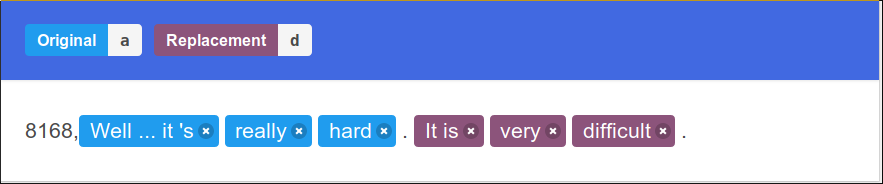
\includegraphics[width=\textwidth]{Figures/doccano.png}
    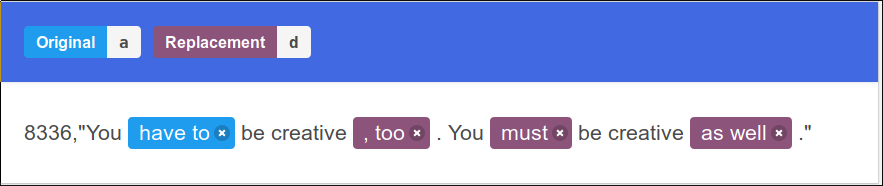
\includegraphics[width=\textwidth]{Figures/doccano2.png}
    \caption{Examples of how the sequence labeling annotation process looked using doccano.}
    \label{fig:doccano-ex}
\end{figure}

Finally, the segments had to be actually marked. I used a tool called \textbf{doccano} to carry out annotations on the paired informal blog post data and formal translated sentences (\cite{doccano2019}). Doccano's sequence labeling task annotator allowed me to select the spans of the sentences which were informal, and separately mark their formal translations. A couple of examples are displayed here at Figure \ref{fig:doccano-ex}. It is important to note that while multiple changes in the same sentences were able to be marked, this was only possible when the replacements were in the formal sentences in the same order that their original counterparts appeared in the source text. Additionally, some of the further syntactic movements were unable to be marked; however, as defined, this was in any case out of the range of the intended dataset, as the aim is to choose selected phrases to translate in-place.

\subsection{Final Characteristics}

Many of the sentences did not have annotations applied to them, either because the translated output did not change or because it changed in a way that no parallel phrases were available (for example, if the output quality was poor). In the end, there were 4848 phrases belonging to 3817 sentences (as some sentences were marked with more than one phrase).

The average Lexical Formality score for the Acrolinx data was calculated as $-0.15$, that is: informal, less informal than the GYAFC source data, more informal than the Microsoft source data and in fact approximately around the level of the Microsoft data when translated with the model from the previous chapter.

\section{Dataset Exploration}

Although the resulting dataset was small, it had the advantage of being human-validated in its entirety. Next, I present some examples from the set and results from testing and exploratory analysis.

\subsection{Examples}

\begin{table}[h]
\centering
 \begin{tabular}{|| p{6cm} | p{6cm} ||} 
 \hline
 Informal Phrase in Sentence & Formal Phrase in Sentence \\ [0.3ex] 
 \hline\hline
 Those lessons include : \textbf{don't} be afraid to chart your own course . & 
    Those lessons include : \textbf{do not} be afraid to chart your own course . \\
\hline
 That is why we are lucky enough to associate muffin tops with people 's waistlines , and to think of trolls not just as the mythological creatures that live under bridges , but also as the \textbf{guys and gals} who like to post mean-spirited comments online . & 
    That is why we are lucky enough to associate muffin tops with people 's waistlines , and to think of trolls not just as the mythological creatures that live under bridges , but also as the \textbf{people} who like to post mean-spirited comments online . \\
\hline
 \textbf{You can also} look at examples from other brands — competitors , or companies in other sectors — that might fire you up to stretch your tone a little bit . & 
    \textbf{It may be possible to} look at examples from other brands — competitors , or companies in other sectors — that might fire you up to stretch your tone a little bit . \\
\hline
 \textbf{And, if} you have been following along , you know that it is also inaccurate . & 
    \textbf{If} you have been following along , you know that it is also inaccurate . \\
\hline
 That may not seem like \textbf{such a big deal} , but the numbers quickly increase when you are referring to lots of different languages . & 
    That may not seem like \textbf{a big deal} , but the numbers quickly increase when you are referring to lots of different languages . \\
\hline
\end{tabular}
\caption{Examples from the resulting Acrolinx Blog Post Dataset.}
\label{acro-data-examples}
\end{table}

Some examples are given in Figure \ref{acro-data-examples}, formatted such that both marked phrases are given in the appropriate place of the original sentence. This also gives a sense of the original informality level of the texts --- casual, but certainly far less informal than the GYAFC data.

It is also clear that not every informal phrase in the original sentences has been identified and translated. Were one to write translations for the informal sentences individually, there are certainly other aspects that would be marked for change: perhaps ``fire you up'' to ``inspire you'', or ``lots of different languages'' to ``a variety of different languages'', as a start. Yet in a sense, this is a natural trade-off when switching from translating a whole sentence to locating and translating a phrase: the focus is to change the segments which can both have an effect on the overall formality of the sentence (make it \textit{less} formal) and have a low risk of scrambling the original meaning.

\subsection{Edit Categorization}

To get a better idea of what changes were covered in the new dataset, I examined the edits, again using doccano, and placed them each into one of eight potential categories. These categories included: when written-out phrases were changed to acronyms (\textbf{acronym}), written-out numbers replaced with digits (\textbf{number}), the removal of qualifiers/intensifiers as ``very'' and ``literally'' (\textbf{qualifier}), the removal of discourse markers like ``but'' and ``and'' (\textbf{discourse}), changing of punctuation (\textbf{punct}), grammatical or syntactic changes (\textbf{grammar}), the expanding of contractions into separate words (\textbf{contraction}), and the changing of words or lexical phrases with formal counterparts (\textbf{lexical}).

\begin{figure}
    \centering
    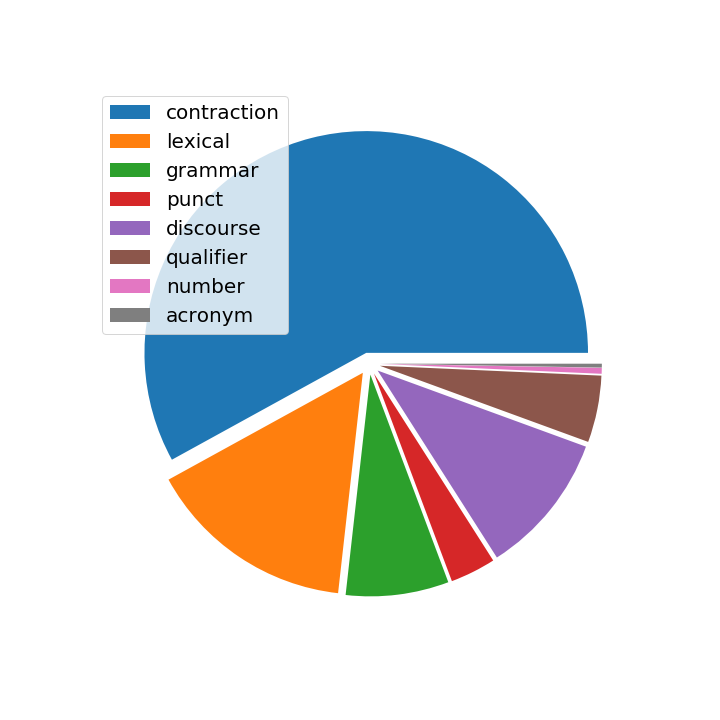
\includegraphics[width = 12cm]{Figures/pie_fig.png}
    \caption{Results of edit classification on the Acrolinx dataset.}
    \label{fig:doccano-edits}
\end{figure}

\begin{table}[h]
\centering
 \begin{tabular}{||c | r | l | l ||} 
 \hline
 Category & \% & Informal Example & Formal Example \\ [0.3ex] 
 \hline\hline
 contraction & 58.0\% & don't & do not \\ 
 \hline
 lexical & 15.2\% & plus & in addition \\
 \hline
 discourse & 10.4\% & So can you answer \textit{[...]} & Can you answer \textit{[...]} \\
 \hline
 grammar & 7.5\% & Go \textit{[...]} & You should go \textit{[...]} \\
 \hline
 qualifier & 4.9\% & absolutely agree & agree \\
 \hline
 punct & 3.3\% & \textit{[...]} with you! & \textit{[...]} with you. \\
 \hline
 number & 0.4\% & 13 & thirteen \\
 \hline
 acronym & 0.3\% & US & United States \\
 \hline
\end{tabular}
\caption{Percentages of each category of edit in the Acrolinx Blog Post Dataset, and examples.}
\label{acro-edits-table}
\end{table}

The results of this task are available in a visual sense in Figure \ref{fig:doccano-edits}, and with more specifics and examples in Table \ref{acro-edits-table}. As can be instantly seen, contractions make up the majority of the edits, likely because for the model which translated them, these were simple changes to pick up on and be consistent with. The changes in grammar were mostly the addition of relativizers or filling of technically incomplete sentences.

These figures are worthwhile to compare with those of Table \ref{pavlick2016table}, which gives the results from a similar effort by \cite{pavlick2016empirical}, due to the difference in domain. Though there is immediately visible overlap in the categories, there are also stark differences. As \cite{pavlick2016empirical} carried out their classification on changes in online debate forum data, there were other categories present that were not found in the Acrolinx blog posts: namely, \textit{normalization}, \textit{spelling} and \textit{capitalization} are examples of changes with, as they are considered linguistic errors, would not be present in professional texts like the Acrolinx blogs. Similarly, the punctuation changes are many more in their data as opposed to these data because the informality that using (for example) more than one exclamation mark brings is too high. The same applies to slang and idioms. That the two largest categories after capitalization and punctuation are ``paraphrase'' and ``delete fillers'', though, is analogous to the two largest after contraction for the Acrolinx data being lexical and discourse.

\section{Takeaway}

I confirmed that not all aspects of informality, as defined by \cite{pavlick2016empirical}, are present in the desired level of informality for this use case, as defined by these data from Acrolinx blog posts. Informality, as should by now be clear, takes on different sets of characteristics in different domains or contexts. With this in mind, I elected to narrow my focus for this project on those characteristics are most relevant and also approachable with machine learning techniques. Certain categories, such as expanding or creating contractions, are more likely to be achievable with rule-based methods. Others, which require deeper semantic understanding, could benefit from these algorithms.

From the selection gathered here, and for the presented reasons, I chose two categories of edits: discourse marker insertion and lexical/phrase replacement. Both had a significant presence in the Acrolinx data edits, and both necessitate understanding of their sentence- or even paragraph-level contexts.